\section{Introduction}

Il s'agit dans ce chapitre d'introduire les probl\'ematiques et m\'ethodologies qui nous guideront dans notre \'etude de l'utilisation de l'asservissement visuel pour les robots parall\`eles \`a c\^ables. Notre objectif est double: il s'agit dans un premier temps d'ajouter des fonctionnalit\'es de saisie et manipulation d'objets \`a nos prototypes existants, et d'am\'eliorer les propri\'et\'es de ces m\^emes prototypes dans un second temps.

Pour cela, nous  \'evoquons dans une premi\`ere section les avantages et inconv\'enients des structures parall\`eles comparativement aux structures en s\'erie. Les sp\'ecificit\'es des manipulateurs \`a c\^ables sont introduites dans une deuxi\`eme section, suivie par un rappel des mod\`eles g\'eom\'etriques et cin\'ematiques des manipulateurs parall\`eles \`a c\^ables. Nous pr\'esentons dans la section suivante le prototype sur lequel nos exp\'erimentations et validations ont \'et\'e effectu\'ees, avant d'introduire quelques notions fondamentales pour la suite.

Apr\`es un rappel des mod\`eles d'asservissement visuel, nous introduirons les sp\'ecificit\'es de notre choix de configuration, dont nous montrerons de quelle mani\`ere il se d\'emarque des travaux existants dans ce domaine pr\'ecis. Nous pourrons alors conclure par l'exposition des probl\'ematiques \`a partir desquelles nous nous sommes propos\'e de mener cette \'etude, ainsi que des choix m\'ethodologiques qui en auront guid\'ee la r\'ealisation.

\subsection{Manipulateurs s\'erie et parall\`eles}

\subsubsection{D\'efinitions}

C'est incontestablement l'industrie qui aura \'et\'e le principal vecteur de d\'eveloppe\-ment de la robotique ces deux derniers si\`ecles. L'introduction des robots dans les usines s'inscrit dans une d\'emarche d'augmentation de la productivit\'e et d'am\'elio\-ration de la manufacture. Cela aura permis d\`es lors de soulager le travailleur humain dans des situations de travail p\'enible et/ou r\'ep\'etitif, et d'augmenter ses comp\'etences en permettant par exemple une pr\'ecision qu'il ne saurait fournir seul, ou la possibilit\'e de d\'eplacer des charges \'elev\'ees. Si la grande diversit\'e que recouvre aujourd'hui le terme de {\it robot} rend extr\^ement difficile l'\'elaboration d'une d\'efinition g\'en\'erique, nous pouvons cependant en d\'eriver des sous-cat\'egories plus faciles \`a appr\'ehender. Parmi celles-ci, nous distinguons en particulier la classe des manipulateurs dont l'objectif sera le d\'eplacement et positionnement d\'objets dans l'espace. Un manipulateur sera constitu\'e de mani\`ere g\'en\'erale d'une base et d\'un organe terminal, reli\'es par une ou plusieurs cha\^ines cin\'ematiques plus ou moins \'elabor\'ees.

Une cha\^ine cin\'ematique est caract\'eris\'ee par une succession de solides reli\'es par des articulations. Les articulations simples peuvent \^etre de nature {\it prismatique} \ref{intro:fig0view0} -- permettant la translation d'un solide par rapport \`a l'autre -- ou {\it roto\"ides} \ref{intro:fig0view1} -- effectuant un mouvement de rotation autour d'un axe donn\'e. Des articulations complexes sont obtenues \`a partir de la combinaison de mouvements prismatiques et/ou roto\"ides : une articulation cylindrique \ref{intro:fig0view2} permet par exemple la combinaison d'un mouvement de translation selon un axe donn\'e et d'un mouvement de rotation autour de ce m\^eme axe ; autre exemple, une articulation sph\'erique \ref{intro:fig0view3} combinera quant \`a elle trois rotations.

\begin{figure}[!ht]
  \centering
      \subfloat[Articulation simple de type prismatique]{\label{intro:fig0view0}
    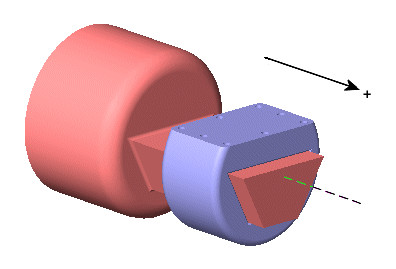
\includegraphics[width=.24\linewidth]{./intro/figures/prismaticJoint.jpg}} \hfill
    \subfloat[Articulation simple de type roto\"ide]{\label{intro:fig0view1}
    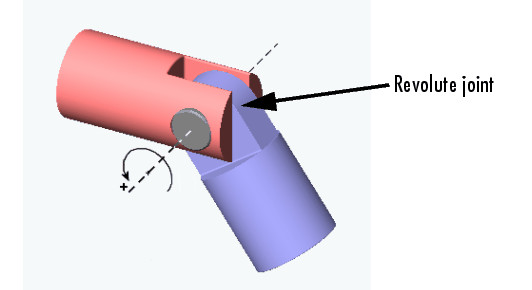
\includegraphics[width=.24\linewidth]{./intro/figures/revoluteJoint.jpg}} \hfill
  \subfloat[Articulation compos\'ee de type cylindrique]{\label{intro:fig0view2}
    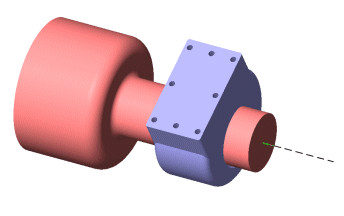
\includegraphics[width=.24\linewidth]{./intro/figures/cylindricalJoint.jpg}} \hfill
  \subfloat[Articulation compos\'ee de type sph\'erique]{\label{intro:fig0view3}
    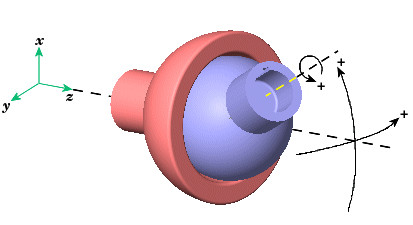
\includegraphics[width=.24\linewidth]{./intro/figures/sphericalJoint.jpg}}
    \caption{\footnotesize{Diff\'erents exemples d'articulations.}}
\label{intro:fig0}
\end{figure}

On appelle {\it coordonn\'ees articulaires} l'ensemble des \'etats de chacune des articulations \`a un instant donn\'e. Lorsque les articulations ne sont pas laiss\'ees libres, leur valeur dans l'{\it espace articulaire} sera contr\^ol\'ee par des {\it actionneurs} : on distinguera donc les {\it articulations actionn\'ees} des {\it articulations libres}. Les coordonn\'ees articulaires sont exprim\'ees dans un espace articulaire propre \`a chaque articulation. Les param\`etres n\'ecessaires \`a l'expression des coordonn\'ees articulaires sont g\'en\'eralement au nombre de 3 pour un point (ses coordonn\'ees dans l'espace cart\'esien) et de 6 pour un solide (position cart\'esienne compl\'et\'ee par trois angles de rotation). Le nombre de param\`etres non fix\'es par la g\'eom\'etrie du robot et n\'ecessaires \`a la description exhaustive des coordonn\'ees d\'une articulation est appel\'e {\it degr\'e de libert\'e}.

De la m\^eme mani\`ere, on parlera des {\it coordonn\'ees op\'erationnelles} pour d\'efinir la position de l'organe terminal, exprim\'ees dans le rep\`ere de l'organe terminal. A nouveau, nous pouvons d\'efinir les degr\'es de libert\'e de l'organe terminal comme le nombre de param\`etres contr\^ol\'es pour le d\'eplacer dans l'espace. Cette notion est \`a distinguer de la mobilit\'e de l'organe terminal, qui correspond aux possibilit\'es de d\'eplacement de l'organe terminal. Si l'on d\'ecide par exemple de contr\^oler les mouvements en rotation, de bloquer deux rotations mais d'en laisser libre une, la mobilit\'e sera de 4, mais le nombre de degr\'es de libert\'es ne sera que de 3.

Enfin, on peut d\'efinir pour chaque segment son {\it degr\'e de connexion} comme \'etant le nombre de solides auxquels il est reli\'e par une articulation libre ou actionn\'ee. Lorsque l'ensemble des segments ont un degr\'e de connexion \'egal \`a 2 \`a l'exception de la base et de l'organe terminal qui ont de degr\'e de connexion \'egal \`a 1, on parle de {\it cha\^ine cin\'ematique ouverte} \ref{intro:fig1view0}. Lorsque l'un des segments au moins (différent de la base) poss\`ede un degr\'e de connexion sup\'erieur ou \'egal \`a 3, nous avons une {\it cha\^ine cin\'ematique ferm\'ee} \ref{intro:fig1view1} \cite{journals/gosselin1989}. Les cha\^ines cin\'ematiques complexes sont constitu\'ees de plusieurs cha\^ines ferm\'ees et/ou ouvertes.

\begin{figure}[!ht]
  \centering
      \subfloat[Sch\'ema d'une cha\^ine cin\'ematique ouverte]{\label{intro:fig1view0}
    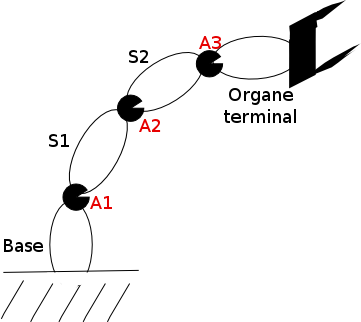
\includegraphics[width=.48\linewidth]{./intro/figures/openchain.png}} \hfill
    \subfloat[Sch\'ema d'une cha\^ine cin\'ematique ferm\'ee]{\label{intro:fig1view1}
    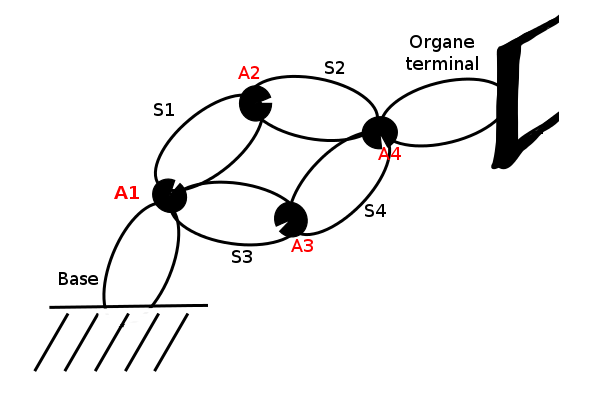
\includegraphics[width=.48\linewidth]{./intro/figures/closedchain.png}}
    \caption{\footnotesize{Exemples de cha\^ines cin\'ematiques ouvertes et ferm\'ees : les $S_i$ repr\'esentent les diff\'erents segments interm\'ediaires, tandis que les $A_i$ correspondent aux articulations. Dans \ref{intro:fig1view0}, tous les segments $S_i$ ont un degr\'e de connexion \'egal \`a 2 ; seuls la base et l'organe terminal ont un degr\'e de connexion \'egal \`a 1. Il est visible dans \ref{intro:fig1view1} que tous les segments \`a l'exception de $S_4$ poss\`edent un degr\'e de connexion \`egal \`a 3.}}
\label{intro:fig1}
\end{figure}

\subsubsection{Architectures s\'eries}

On appelle {\it robot série} un système constitué d'{\bf une chaîne cinématique ouverte dont chaque segment est relié au suivant par une articulation simple} \ref{intro:fig2}. Longtemps dominants dans l'industrie, les robots séries ont pu être privilégiés grâce aux deux caractéristiques suivantes :
\begin{itemize}
 \item sous certaines conditions, le modèle cinématique inverse des robots séries peut être résolu analytiquement \cite{pieper1968kinematics}
 \item leur espace de travail peut rapidement devenir assez conséquent.
\end{itemize}

\begin{figure}[!ht]
  \centering
      \subfloat[Robot série présentant 3 articulations rotoïdes]{\label{intro:fig2view0}
    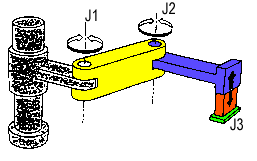
\includegraphics[width=.48\linewidth]{./intro/figures/serialrobot01.png}} \hfill
    \subfloat[Robot série présentant 3 articulations prismatiques]{\label{intro:fig2view1}
    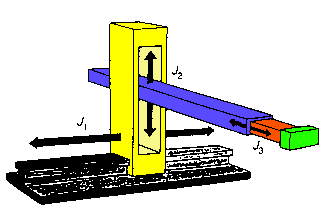
\includegraphics[width=.48\linewidth]{./intro/figures/serialrobot02.png}}
    \caption{\footnotesize{Exemples de robots séries}}
\label{intro:fig2}
\end{figure}

Une architecture série présente toutefois plusieurs inconvénients non négli\-gea\-bles dans un contexte industriel tels que :
\begin{itemize}
 \item chaque segment et articulation porte la charge de tous ceux qui leur succèdent dans la chaîne cinématique. En particulier, cela affaiblit la dynamique lors de l'actionnement des articulations : segments et articulations doivent être rigidifiés, ils sont donc plus lourds, 
 \item les erreurs se propagent de segments en segments ; la précision tout comme la répétabilité du manipulateur en sont affectées,
 \item les charges manipulables ne peuvent être excessives, car elles seront supportées par l'ensemble des segments et articulations.
\end{itemize}

Ainsi, une architecture série impose souvent un dispositif imposant, dont la précision, la dynamique et la faible capacité de charges se révèleront insuffisants pour un grand nombre de tâches requises en particulier par l'industrie moderne.

Une alternative possible consiste en l'utilisation de chaînes cinématiques fermées permettant
\begin{itemize}
 \item une répartition des charges (segment ultérieurs et poids de l'objet manipulé),
 \item une compensation des erreurs entre chaque ``branche'' de la chaîne cinéma\-tique fermée,
 \item une plus grand flexibilité des articulations, impliquant une dynamique plus grande.
\end{itemize}

Les architectures parallèles en particulier présentent une des implémentations possibles de chaînes cinématiques fermées, et leurs caractéristiques -- sur lesquel\-les nous allons nous pencher par la suite -- ont contribué à ce qu'elles s'installent progressivement dans le paysage de la robotique.


\subsubsection{Architectures parallèles}

Une définition des robots parallèles est donnée dans \cite{merlet1997robots} :\\
{\it Un manipulateur parallèle est constitué d’un organe terminal à $n$ degrés de li\-berté et d’une base fixe, reliés entre eux par au moins deux chaînes
cinématiques indépendantes, la motorisation s’effectuant par $n$ actionneurs simples.}\\

Parmi les exemples les plus cités dans la littérature, nous trouvons la plateforme de Gough-Stewart \cite{1956:Gough}, \cite{1965:Stewart} et le robot Delta \cite{1988:Clavel}.

Initialement développée pour des applications dans l'industrie automobile \ref{intro:fig3view0}, la plateforme de Gough-Stewart a par la suite été utilisée dans des applications diverses au rang desquelles les simulateurs de vols \ref{intro:fig3view1}. Sa plateforme mobile peut être déplacée selon 6 degrés de liberté (translations $+$ rotations) à l'aide de six jambes indépendantes actionnées par des vérins pneumatiques. Les articulations la reliant à la base (cardan) et à la plateforme (rotule) sont quant à elles laissées libres.

Le robot Delta \ref{intro:fig3view2} permet un déplacement de sa platforme selon les trois degrés de liberté correspondant aux translations. Trois jambes sont utilisées pour cela, chacune étant reliée à la base par une articulation rotoïde à un levier, lui-même relié à un segment parallélogramme par une seconde articulation rotoïde, une troisième articulation rotoïde liant ce segment à l'organe terminal. Il peut atteindre des vitesses allant jusqu'à 10 m/s et des accélérations jusqu'à 20G, ce qui le rend particulièrement adapté pour des tâches de conditionnement. 

\begin{figure}[!ht]
  \centering
      \subfloat[Plateforme de Gough utilisée dans une usine de pneumatiques]{\label{intro:fig3view0}
    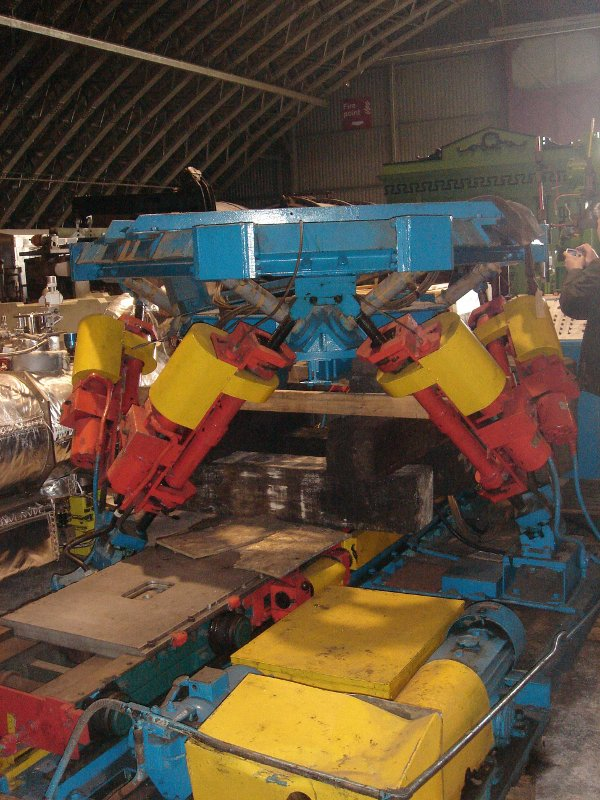
\includegraphics[width=.34\linewidth]{./intro/figures/parallelrobot01.jpg}} \hfill
    \subfloat[Plateforme de Gouch-Stewart utilisée pour des simulateurs de vols]{\label{intro:fig3view1}
    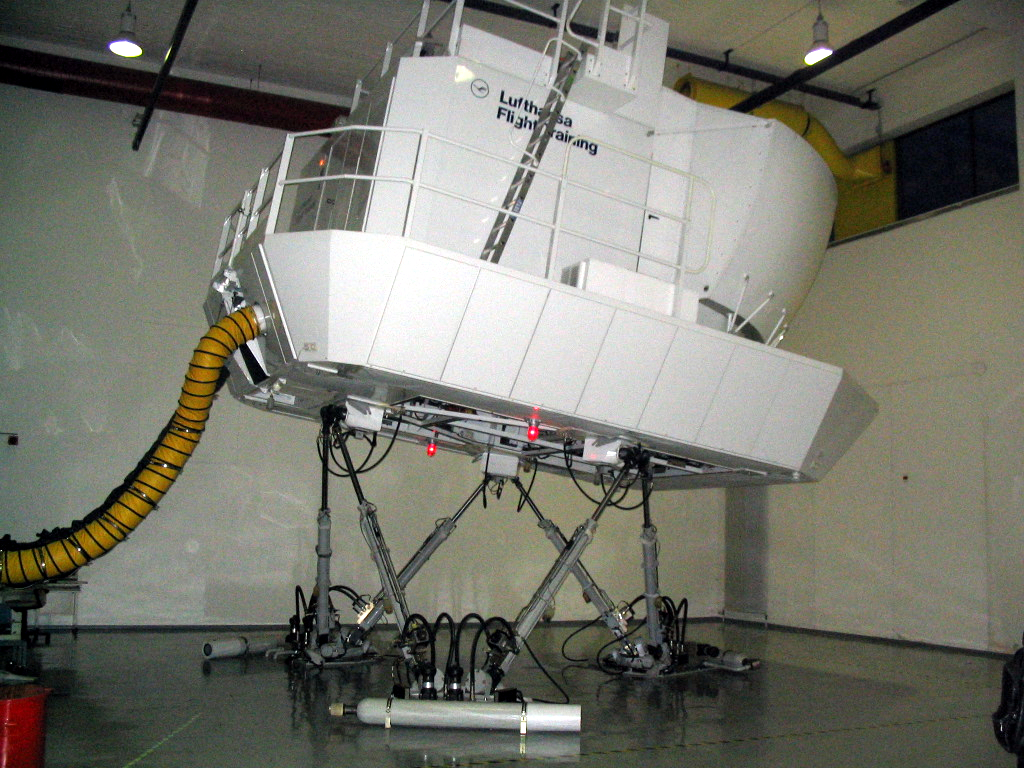
\includegraphics[width=.60\linewidth]{./intro/figures/parallelrobot02.jpg}} \\
    \subfloat[Robot Delta, particulièrement adapté aux tâches de ``pick and place'']{\label{intro:fig3view2}
    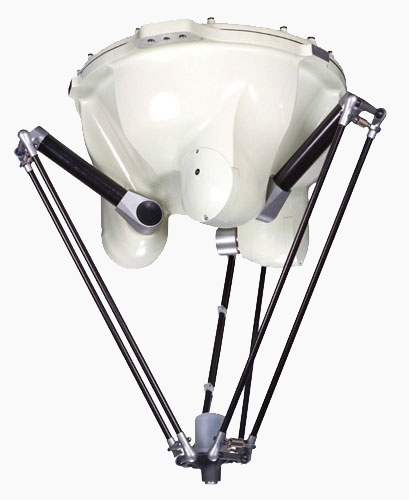
\includegraphics[width=.45\linewidth]{./intro/figures/parallelrobot03.jpg}}
    \caption{\footnotesize{Exemples de robots parallèles}}
\label{intro:fig3}
\end{figure}

De manière générale, les manipulateurs parallèles présentent les caractéristi\-ques sui\-vantes permettant de les comparer avantageusement aux manipulateurs séries :
\begin{itemize}
 \item une précision accrue par un mécanisme de {\bf compensation} des erreurs entre les différentes chaînes cinématiques (autrement appelées {\it jambes}),
 \item une capacité de charge élevée due à la {\bf répartition} de la charge sur les différentes jambes,
 \item une grande rigidité provenant de la taille réduite des chaînes cinématiques,
 \item une dynamique élevée conséquente de la {\bf coopération} des différentes jam\-bes dans le positionnement de l'organe terminal.
\end{itemize}

Toutefois, les mécanismes parallèles possèdent plusieurs inconvénients qui doivent être pris en compte lors du choix d'une architecture :
\begin{itemize}
 \item des modèles géométriques directs complexes, dont la résolution algébrique n'est pas toujours possible,
 \item existence de singularités pouvant conduire à une perte de contrôle du manipulateur,
 \item la répartition entre les jambes des forces appliquées sur la plateforme n'est qu'en de très rares cas uniforme ; certaines positions peuvent affecter le contrôle, la rigidité et la précision du mécanisme,
 \item un espace de travail limité inférieur à l'intersection des espaces atteignables par chaque jambe,
\end{itemize}

On peut distinguer deux types de stratégies concernant la résolution des modèles géométriques directs : une première consiste à utiliser des outils numé\-riques tels l'analyse par intervalles \cite{Merlet04solvingthe}, une seconde à choisir une géométrie pour laquelle une résolution algébrique est possible \cite{2003:Krut1}. Concernant les diverses singularités, la difficulté peut être contournée par exemple par l'utilisation de méthodes de planification de trajectoires \cite{2008:Chen.Chi}, \cite{1998:Dasgupta.Mruthyunjaya} ou à nouveau grâce à la détermination de géométries adaptées \cite{w1994:DiCaprioStanisic}. Il est évidemment possible de renforcer la structure des jambes et des actionneurs pour assurer la rigidité des chaînes cinématiques en toutes circonstances ; il est également possible, lorsque pour une position de l'organe terminal donnée, plusieurs configurations articulaires sont possibles, de choisir celle qui garantit le meilleur fonctionnement du robot \cite{2002:Verhoeven.Miller} : ainsi, l'existence de plusieurs solutions au modèle géométrique direct devient un avantage plus qu'en inconvénient, en ce que cela permet d'optimiser certains critères -- ici la répartition des forces exercées sur la plateforme -- pour un meilleur contrôle du robot.

La problématique d'un espace de travail réduit subsiste et reste une contrainte forte des mécanismes parallèles. Bien qu'ils présentent des spécificités propres pour chacune des caractéristiques déjà évoquées (rigidité, précision, charge nominale, \dots), la classe des robots parallèles à câbles a principalement été développée afin de conserver les propriétés des robots parallèles pour des applications exigeant un mécanisme léger possédant un volume de travail de taille conséquente, par exemple pour intervenir lors de catastrophes naturelles ou dans des environnements toxiques \cite{1992:Albus.Bostelman.ea}. C'est à l'étude et au développement de cette catégorie paticulière de manipulateurs que seront consacrés l'essentiel des travaux présentés dans ce manuscrit et pour laquelle nous emploierons désormais indistinctement les noms de robots, manipulateurs, robots parallèles à câbles ou CDPR (pour {\it cable-driven parallel robot}).

\subsection{Les manipulateurs parallèles à câbles}

Les manipulateurs parallèles à câbles présentent une structure en chaînes cinéma\-tiques fermées, la base et la plateforme étant reliées exclusivement au moyen de câbles. Les actionneurs sont en général positionnés sur la base et leur fonction consiste à contrôler la longueur des câbles. On peut donc les considérer comme des articulations prismatiques dont la course peut s'avérer rapidement atteindre des longueurs remarquables, augmentant considérablement l'espace de travail du manipulateur.

Afin de contrôler la longueur des câbles, plusieurs types d'articulations peuvent être utilisés, parmi lesquels :
\begin{itemize}
 \item des poulies actionnées par des moteurs rotatifs autour desquelles s'enrou\-leront ou se dérouleront les câbles \ref{intro:fig4view0} ; cette solution a l'avantage d'être extrêmement légère et aisément déployable, mais présente l'inconvénient du contrôle de la longueur enroulée lorsque le câble n'est pas guidé : il est dès lors impossible d'éviter une superposition lors de l'enroulement, et dès lors de connnaître le diamètre réel pour une couche donnée.
 \item les câbles sont reliés à des plateformes se déplaçant sur des rails, ce qui permet d'en contrôler la longueur \cite{merlet2008} ; la multiplication des plateformes en mouvement permet en théorie un contrôle plus rapide et plus précis \ref{intro:fig4view1}. 
\end{itemize}

\begin{figure}[!ht]
  \centering
      \subfloat[L'enroulement et le déroulement des câble sse fait ici par un système de poulie actionnée par un moteur]{\label{intro:fig4view0}
    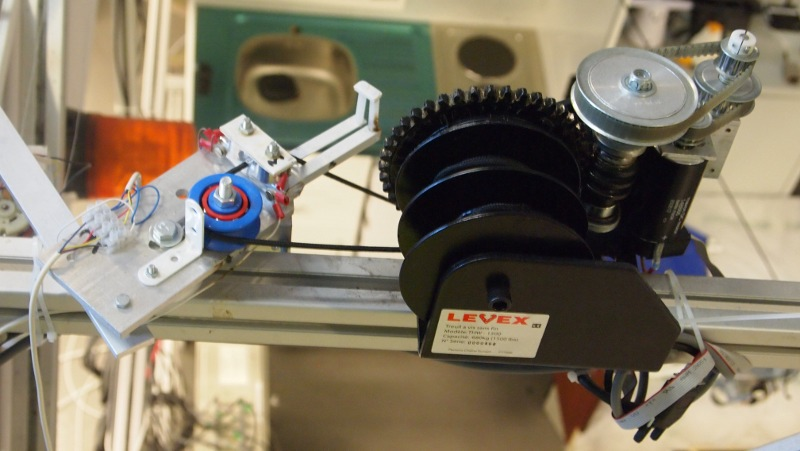
\includegraphics[width=.55\linewidth]{./intro/figures/winchesactuator.jpg}} \hfill
    \subfloat[Les câbles sont fixés à des plateformes pouvant se déplacer linéairement sur des rails, permettant un contrôle de la longueur]{\label{intro:fig4view1}
    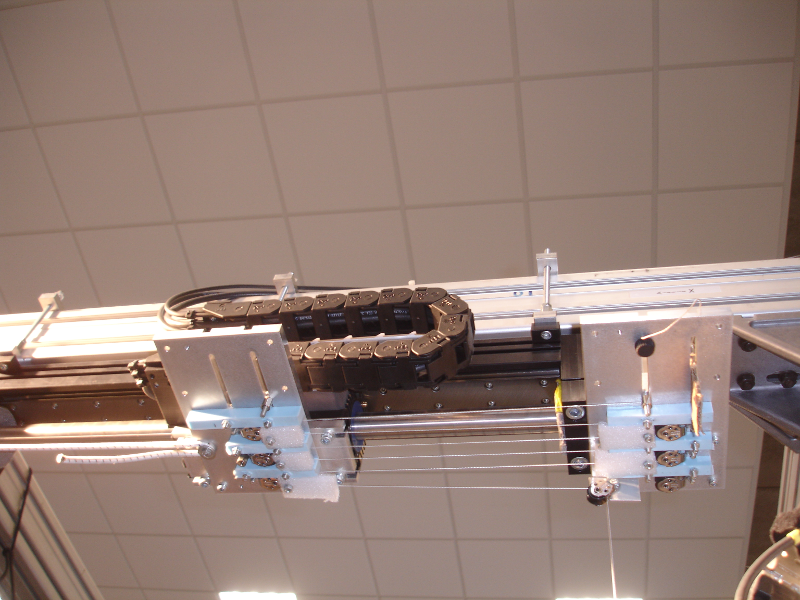
\includegraphics[width=.42\linewidth]{./intro/figures/linearactuator.png}}
    \caption{\footnotesize Deux types d'articulations et d'actionnement pour un robot à câble}
\label{intro:fig4}
\end{figure}

Toutefois, quelque-soit le type d'articulation et d'actionnement choisis, la force que peut exercer un seul câble sur l'organe terminal est nécessairement unilatérale : un câble seul peut tirer, mais ne peut pas pousser la plateforme. Il faut donc, pour pouvoir contrôler le mouvement dans son intégralité, que les câbles travaillent en opposition. Il a ainsi été montré que $n+1$ câbles au minimum sont requis pour assurer le contrôle de $n$ degrés de liberté. On peut cependant considérer la gravité comme une force unilatérale et la représenter comme un câble virtuel : il est ainsi possible de n'utiliser que $n$ câbles pour $n$ degrés de liberté.

On distingue donc deux types de configurations pour un robot parallèle à câbles :
\begin{itemize}
 \item en {\it configuration pleinement contrainte} \ref{intro:fig5view0}, les câbles travaillent en opposition et $n+1$ sont nécessaires pour assurer des déplacements et l'application de forces correspondant à $n$ degrés de liberté.
 \item en {\it configuration suspendue} \ref{intro:fig5view1}, la gravité agit comme un câble virtuel : les câbles sont fixés généralement au point le plus haut du dispositif, et $n$ suffisent pour déplacer et orienter l'organe terminal selon $n$ degrés de liberté. On retrouve parfois ce type de configuration dans la littérature sous le nom de {\it grue} ou {\it crane}. Pour exemple, le manipulateur {\it Nist Spider} \cite{1992:Albus.Bostelman.ea} mentionné précédemment présentait une configuration suspendue.
\end{itemize}

\begin{figure}[!ht]
  \centering
     \subfloat[Exemple de configuration pleinement contrainte]{\label{intro:fig5view0}
    
\includegraphics[width=.50\linewidth]{./intro/figures/robot_cdpr_noncrane.jpg}} \hfill
    \subfloat[Exemple de configuration suspendue]{\label{intro:fig5view1}
    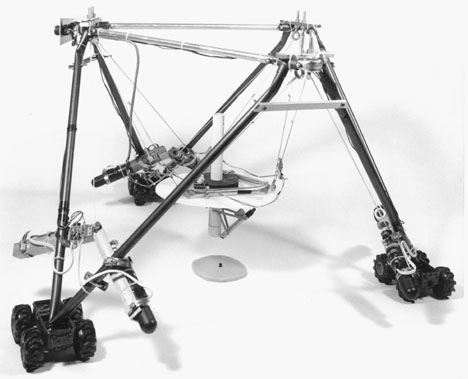
\includegraphics[width=.40\linewidth]{./intro/figures/robot_cdpr_crane.jpg}}
    \caption{\footnotesize Deux configurations possibles pour un robot parallèle à câble}
\label{intro:fig5}
\end{figure}

Une caractéristique sensible des manipulateurs parallèles à câbles qui les différencie des manipulateurs parallèles classiques est la {\bf non-rigidité des jam\-bes}. Sous certaines conditions, un ou plusieurs câbles peuvent être détendus, ce qui a pour effet 1/ de modifier leur géométrie, 2/ ils n'exercent plus de force sur la plateforme. Pour certaines configurations, il peut d'ailleurs être montré qu'il existera toujours au moins un câble détendu quelque-soit la position de l'organe terminal et les forces exercées sur celui-ci \cite{2011:Carricato.Merlet}. Le prototype sur lequel nous avons conduit nos expériences présentant ce type de comportement, nous reviendrons plusieurs fois largement sur ce point.

Enfin, lorsqu'un câble est sous tension, un modèle complet doit pouvoir prendre en compte son élasticité, sa masse, \dots qui affecteront sa longueur réelle et donc la précision avec laquelle le manipulateur est contrôlé.

Comparativement donc aux robots parallèles classiques, les robots parallèles à câbles présentent les caractéristiques suivantes :
\begin{itemize}
 \item la structure parallèle permet de conserver les propriétés de compensation des erreurs, de répartition des charges et des efforts, de coopération des chaînes cinématique pour l'exécution d'un mouvement
 \item l'espace de travail est considérablement agrandi malgré la conservation de la légèreté du dispositif.
 \item la modélisation des câbles ainsi que le choix des articulations et actionneurs complexifient le modèle du robot ; une simplification du modèle en négligeant certaines de ces caractéristiques est alors source d'imprécisions qui devront être intégrées au schéma de contrôle.
 \item l'unilatéralité des forces suppose que nous puissions nous retrouver dans une situation avec un ou plusieurs câbles détendus. Nous verrons cependant qu'il est possible de prendre avantage de cette situation afin d'amélio\-rer le contrôle de l'organe terminal pour une trajectoire donnée.
\end{itemize}

Après avoir introduit quelques notations utiles, nous allons à présent décrire les modèles géométriques directs et indirects, cinématiques ainsi que l'équilibre statique pour les robots parallèles à câble. Ceci nous permettra de lister tant que faire se peut l'ensemble des difficultés posées par ce type de manipulateur et auxquelles nous avons été confrontées dans le cadre de ces recherches.

\subsubsection{Notations}

\begin{itemize}
 \item $R_b$ : référentiel de la base
 \item $R_e$ : référentiel de l'organe terminal
 \item $A_i$ : point d'attache du $i^{\hbox{ème}}$ câble à la base ; le terme de {\it point de sortie} sera également utilisé.
 \item $B_i$ : point d'attache du $i^{\hbox{ème}}$ câble à l'effecteur
 \item $C$ : un point arbitraire de l'effecteur utilisé comme référence pour sa position
 \item $\rho_i$ : longueur réelle du câble $i$
 \item $l_i$ : longueur déroulée du câble $i$
 \item $\bf {\mathcal F}$ : vecteur des forces exercées sur l'effecteur
 \item $\bf J$ : jacobienne du robot
\end{itemize}
Enfin, on utilisera la notation $J^{-1}$ pour exprimer la jacobienne inverse, et $J^{-T}$ sera utilisé comme raccourci de notation pour sa transposée.

\subsubsection{Modèle géométrique indirect}

Le modèle géométrique indirect consiste à déterminer les coordonnées articulaires à partir des coordonnées opérationnelles. Dans le cas des robots parallèles à câbles, les coordonnées articulaires correspondent aux longueurs des câbles. Lorsque ceux-ci sont tendus, cette longueur doit être égale à la distance entre les points de sortie $A_i$ et le point d'attache à la plateforme $B_i$. Dans le cas où le câble est détendu, la longueur sera supérieure à cette distance \ref{intro:fig5view0}.\\

\begin{figure}[!ht]
  \centering
      \subfloat[Forme d'un câble dont la tension serait nulle]{\label{intro:fig6view0}
    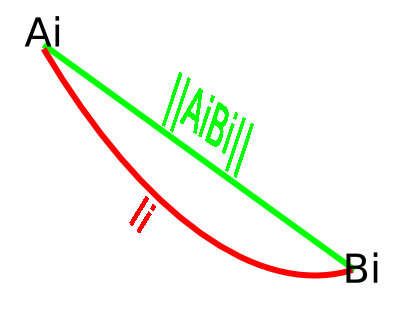
\includegraphics[width=.45\linewidth]{./intro/figures/nulltensionwire.png}} \hfill
    \subfloat[Câble élastique sur lequel est appliquée une tension positive : la longueur réelle diffère de la longueur déroulée]{\label{intro:fig6view1}
    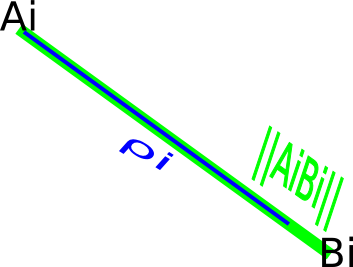
\includegraphics[width=.45\linewidth]{./intro/figures/positivetensionwire.png}} \\
    \caption{\footnotesize{Dans le cas d'un câble détendu (tension nulle), la longueur déroulée sera supérieure à la distance entre les deux points d'attache ; de plus, la forme du câble sera telle qu'il y a risque d'intersection avec d'autres câbles, l'environnement, \dots. Dans le cas d'un câble élastique tendu (tension strictement positive), la longueur déroulée sera inférieure à la distance entre les points d'attache correspondant à la longueur réelle du câble}}
\label{intro:fig6}
\end{figure}

Nous partons donc des relations suivantes :
\begin{eqnarray}
\rho_i &=& ||A_i B_i||, \hbox{ if } \tau_i > 0 \\ 
\rho_i &\geq& ||A_i B_i||, \hbox{ if } \tau_i = 0
\label{intro:eq1}
\end{eqnarray}

Notons que les câbles peuvent être élastiques : ainsi, lorsqu'ils sont en tension, la longueur déroulée pourra être inférieure à la distance $d_i = ||A_i B_i||$ \ref{intro:fig5view1}. Plusieurs modèles de câbles peuvent être utilisés pour estimer le rapport entre la longueur réelle et la longueur déroulée \cite{1974IrvineCaughey}, \cite{2006:Kozak.ea}. A titre d'exemple, le modèle linéaire suivant peut-être utilisé lorsque la masse des câbles est négligeable devant les forces appliquées sur la plateforme :
$$\tau_i = \kappa(\rho_i - l_i)$$
où $\kappa$ est un coefficient correspondant à la raideur linéique du câble.

Pour être complet, le modèle géométrique inverse doit donc envisager toutes les configurations possibles de répartition de tension dans les câbles et, le cas échéant, intégrer la modélisation des câbles dans le processus de résolution. Il est donc fondamental de vérifier la tension exercée dan chaque câble, et en avoir une estimation suffisante selon le modèle d'élasticité des câbles choisi. Nous parlerons donc avec \cite{Carricato-2010-06b} de modèle géométrico-statique indirect, requérant l'étude de l'équilibre statique.

\subsubsection{Equilibre statique}

On dit pour un solide au repos qu'il est en équilibre statique si l'ensemble des forces exercées s'annulent de manière à ce qu'il ne puisse générer ni de mouvement dans l'espace ni de rotation :

\begin{equation}
\mathcal {\bf F}_{\hbox{ext}} = \vec {\bf 0}
\label{intro:eq2}
\end{equation}

L'hypothèse est émise selon laquelle les forces de frottement, de résistance, \dots sont négligeables. Nous ne prenons en compte dès lors que la force de gravité appliquée sur la plateforme, les efforts exercés sur chacun des câbles, ainsi que les couples qui doivent être nuls.

Soit $W_i$ le torseur d'efforts correspondant aux efforts et couples exercés sur le câble $i$ :
\begin{equation}
W_i = ({\bf u}_i^T, (\mathcal R {\bf b}_i \times {\bf u}_i)^T)^T
\label{intro:eq3}
\end{equation}
avec $u_i = \frac{A_iB_i}{\rho_i}$ la direction dans laquelle l'effort est exercé (de $B_i$ vers $A_i$).

En posant $\mathcal F = [0, 0, -mg, 0, 0, 0]^T$ pour le câble virtuel modélisant la force de gravité exercée sur la plateforme, \ref{intro:eq3} devient :
\begin{equation}
\mathcal F + {\bf W} {\bf \tau} = 0
\label{intro:eq4}
\end{equation}
avec ${\bf \tau} = (\tau_1, \tau_2, \dots)^T$ le vecteur d'efforts et ${\bf W}$ la matrice composée des vecteurs des forces appliquées sur les câbles.

En posant ${\bf J}^{-T} = - {\bf W}$, la relation \ref{intro:eq5} s'écrit encore :
\begin{equation}
\mathcal F = {\bf J}^{-T} {\bf \tau}
\label{intro:eq5}
\end{equation}
où $J^{-1}$ est une matrice que l'on appelle {\it jacobienne inverse}.

La détermination des tensions correspondantes à l'équilibre statique correspond à la résolution du système posé par \ref{intro:eq5}.

\subsubsection{Modèle géométrico-statique inverse (ou {\it MGSI})}

Soit $m$ le nombre de câbles et $n$ le nombre de degrés de liberté du robot. Le {\it MGSI} est un problème à $2m$ inconnues ($m$ longueurs + $m$ tensions) et à $n+m$ équations (le modèle géométrique indirect en fournit $m$ et l'équilibre statique en donne $n$). Si $m > n$, est système est sous-contraint. La stratégie consiste dans ce cas à considérer tous les $n$-uplets de câbles et vérifier pour chacun la positivité des tensions à l'équilibre statique.

Doivent être considérées également les situations où l'équilibre n'est réalisé qu'avec $m < n$ câbles en tension positive. C'et une situation pour laquelle le système est sur-contraint et peut ne présenter aucune solution. Il peut toutefois être résolu pour un {\it mode degradé du système}, à savoir la perte de contrôle d'un ou plusieurs degrés de liberté. On parlera alors de {\it singularité} pour caractériser le fait que dans cette position, le contrôle de la plateforme n'est plus possible pour l'ensemble des degrés de liberté du robot.

On comprend ici que le choix d'utiliser des câbles redondants peut être dicté tout autant par des stratégies d'optimisation de la répartition des tensions (lorsque c'est possible) que par la volonté de garantir en tout point de l'espace de travail l'existence d'une solution au {\it MGSI} pour laquelle l'ensemble des degrés de liberté de la plateforme est parfaitement contrôlé.

On peut remarquer enfin que lorsque la composition des câbles est telle que leur élasticité est négligeable pour un espace de travail donné, ils peuvent être assimilés à des jambes rigides et l'on se retrouve dès lors dans une situation équivalente à la résolution du {\it MGI} classique des robots parallèles rigides dont on retrouvera une étude complète dans \cite{merlet1997robots}.

\subsubsection{Modèle géométrico-statique direct}

